\documentclass[12pt]{article}
\usepackage{geometry}                % See geometry.pdf to learn the layout options. There are lots.
\geometry{letterpaper}                   % ... or a4paper or a5paper or ... 
%\geometry{landscape}                % Activate for for rotated page geometry
\usepackage[parfill]{parskip}    % Activate to begin paragraphs with an empty line rather than an indent
\usepackage{daves,fancyhdr,natbib,graphicx,dcolumn,amsmath,lastpage,url}
\usepackage{amsmath,amssymb,epstopdf,longtable}
\usepackage[final]{pdfpages}
\DeclareGraphicsRule{.tif}{png}{.png}{`convert #1 `dirname #1`/`basename #1 .tif`.png}
\pagestyle{fancy}
\lhead{CE 3354 -- Engineering Hydrology}
\rhead{FALL 2024}
\lfoot{ES1}
\cfoot{}
\rfoot{Page \thepage\ of \pageref{LastPage}}
\renewcommand\headrulewidth{0pt}



\begin{document}
\begin{center}
{\textbf{{ CE 3354 Engineering Hydrology} \\ {Exercise Set 2 : By-Hand Solution}}}
\end{center}

This solution is a by-hand approach; GIS based approach will be in a seperate document, there is considerable overlap - either way is fine, although in modern practice, its far more likely you will use GIS tools.  

Some of the original figures are omitted to reduce the file size.

\section*{\small{Exercises}}

\begin{enumerate}
\item Using a GIS (i.e. QGIS) load an OpenStreetMap layer and locate the ``Assessment Point'' 

\textbf{By-Hand Approach}

For a by-hand approach this step coule be accompliehed by finding the location on Google Earth, then convert to UTM coordinates (for later GIS usage).

Figure \ref{fig:GEProLocate} is a screen capture of using Google Earth to capture Lat-Lon location coordinates.

\begin{figure}[h!] %  figure placement: here, top, bottom, or page
   \centering
   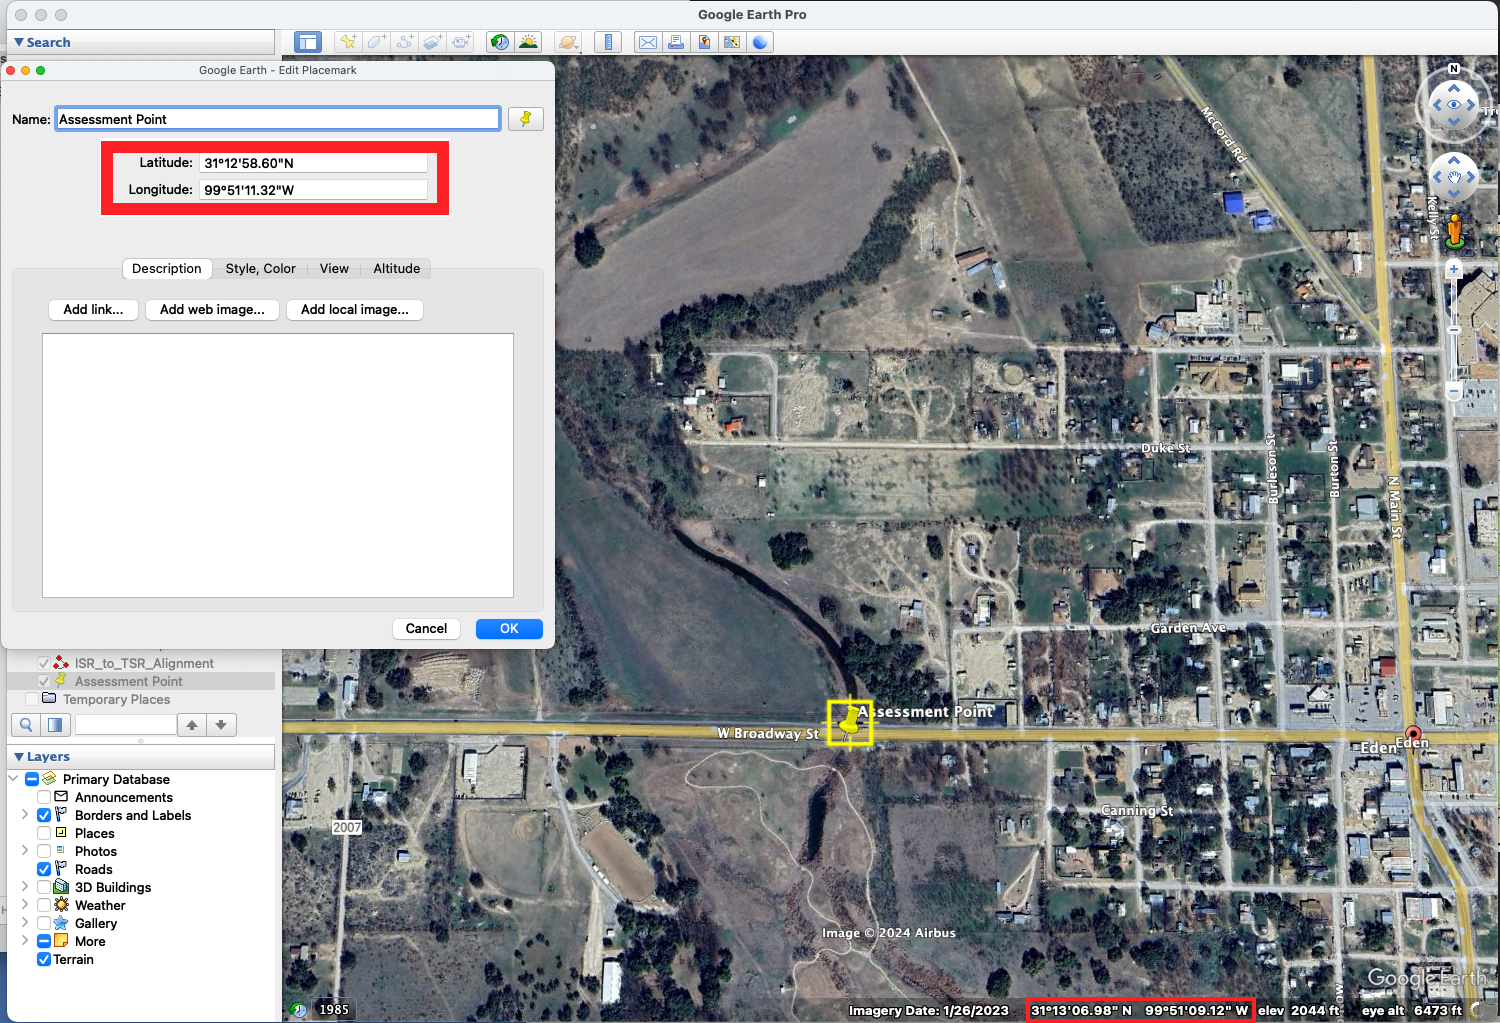
\includegraphics[width=4in]{GEProLatLon.png} 
   \caption{Assessment point coordinates (in DDDMMSS.SS)}
   \label{fig:GEProLocate}
\end{figure}

Figure \ref{fig:DMS2UTM} is a screen capture showing conversion from DMS coordinates into UTM (Zone 14 Texas).

\begin{figure}[h!] %  figure placement: here, top, bottom, or page
   \centering
   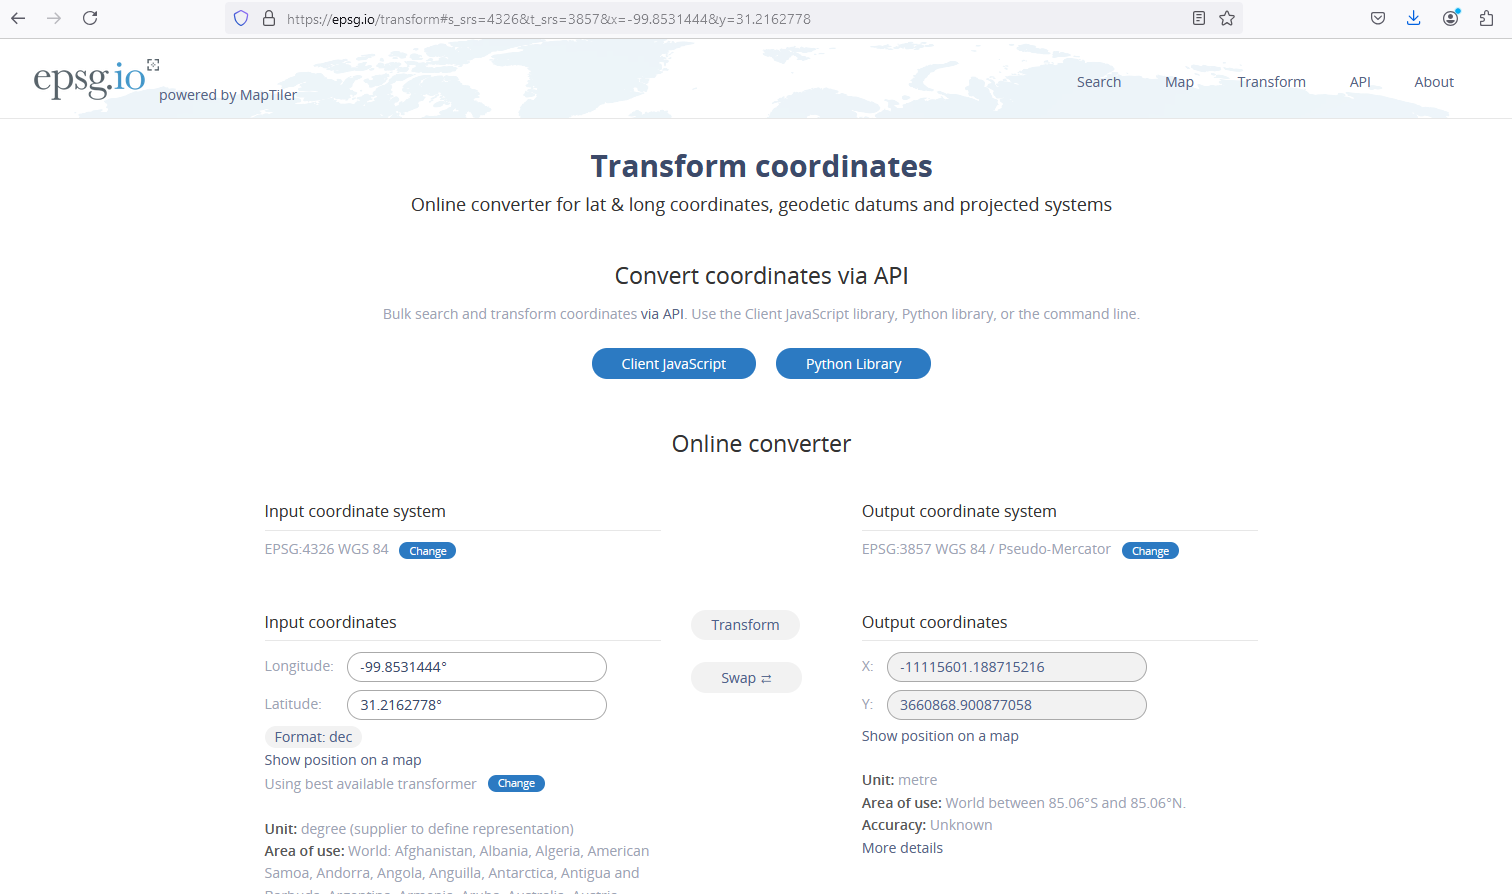
\includegraphics[width=4in]{CoordinateTransform.png} 
   \caption{Assessment point coordinate transformation for GIS use (in UTM Zone 14) (Read the USAF excerpt on topographic maps to learn about UTM coordinate system)}
   \label{fig:DMS2UTM}
\end{figure}

\clearpage

\item Draw the boundary of the entire watershed area (i.e delineate the watershed)

\textbf{By-Hand Approach}

Figure \ref{fig:ES2-WatershedDelineated-2} shows the result of watershed delineation using a combination of a grid and topographic interpretation.   The entire system is divided into three subcatchments based on the presence of the two regulating structures (earth berms with riser pipe outlets) - the intial GIS analysis will not be able to select out the two regulating structures automatically, and the analyst has to intervene - hence a crude by-hand approach is allways useful. 

\begin{figure}[h!] %  figure placement: here, top, bottom, or page
   \centering
   \includegraphics[width=5in]{ES2-WatershedDelineated-2.png} 
   \caption{Study Area -- with grid overlay, outlet (Blue Dot), and subcatchments identified.  Various flow paths are indicted in transparent blue.  Red arrows indicate downslope directions.}
   \label{fig:ES2-WatershedDelineated-2}
\end{figure}

\clearpage
%%%%%%%%%%%%%%%%%%%%%%%%%%%%%%%%%%%%%%%%%%%%%%%%%%%%%%%%%%%%%%%%%%%%%%%%%%%%%%%%%%

\item Determine the drainage area of the watershed in square miles.

\textbf{By-Hand Approach}
The entire watershed area can be computed by manual or numerical planimetry, or counting the squares contained within the watershed.   Each square on the figure represents an area of approximately 0.01 mi$^2$.

Figure \ref{fig:ES2-WatershedArea-2} is a scanned image of the watershed with various square counts.  The estimated area is 16.93 square miles.   This is the total drainage area including all catchments.  The sub-catchment area determinations portions are not shown on this exhibit.  

\begin{figure}[h!] %  figure placement: here, top, bottom, or page
   \centering
   \includegraphics[width=6in]{Scan.png} 
   \caption{Study Area -- with grid overlay, outlet (Blue Dot), and subcatchments identified.  Various flow paths are indicted in transparent blue.  1,693 Squares counted to estimate watershed area.}
   \label{fig:ES2-WatershedArea-2}
\end{figure}

\clearpage
%%%%%%%%%%%%%%%%%%%%%%%%%%%%%%%%%%%%%%%%%%%%%%%%%%%%%%%%%%%%%

\item Find the coordinates of the two outlet risers for the two SCS impoundments in the area; GoogleEarth might be helpful; a proper USGS Topographic map would also be helpful.  You will need these coordinates for future homework/project.

\textbf{By-Hand Approach}
This step can be accomplished using Google Earth (or similar tool) as illustrated

For the West reservoir the location is found in Google Earth as shown in Figure \ref{fig:WestBasin}.  The elevations are taken from the USGS 7.5 minute Topographic Map (the supplied basemap) and confirmed in Google Earth - the Google Earth are within a foot or two of the paper map values.

\begin{figure}[h!] %  figure placement: here, top, bottom, or page
   \centering
   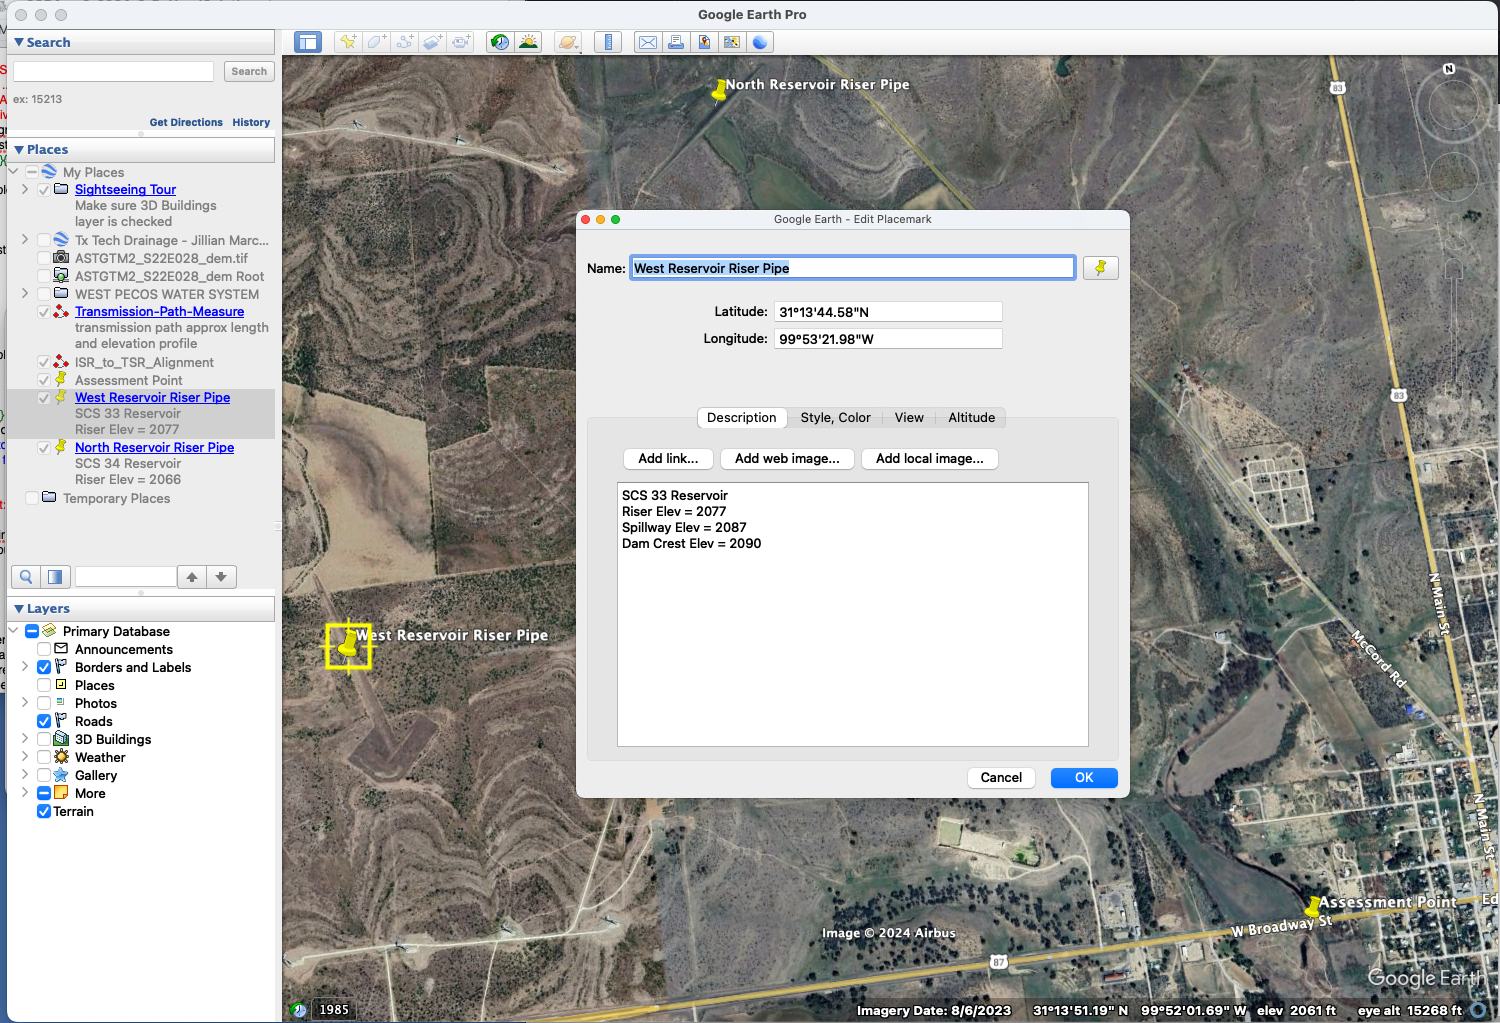
\includegraphics[width=3in]{WestReservoir.png} 
   \caption{West Reservoir riser pipe location, elevations from USGS 7.5 minute basemap, verfied on Google Earth as "close enough"}
   \label{fig:WestBasin}
\end{figure}

Then a coordinate transformation as shown in Figure \ref{fig:WestCoordinates}

\begin{figure}[h!] %  figure placement: here, top, bottom, or page
   \centering
   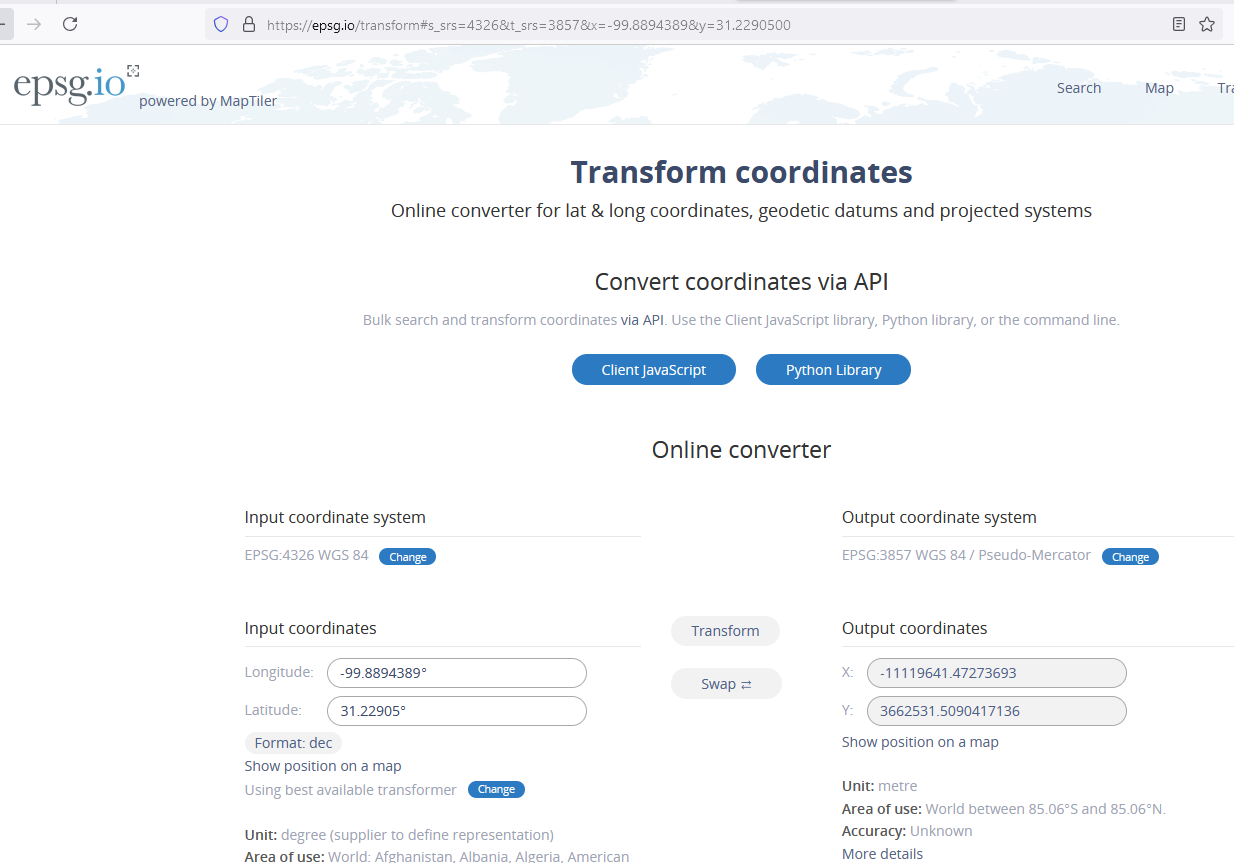
\includegraphics[width=3in]{WestCoordinates.png} 
   \caption{West Reservoir DMS to UTM conversion}
   \label{fig:WestCoordinates}
\end{figure}

\clearpage
%%%%%%%%%%%%%%%%%%%%%%%%%%%%%%%%%%%%%%%%%%%%%%%%%%%%

For the North reservoir the location is found in Google Earth as shown in Figure \ref{fig:NorthBasin}.  The elevations are taken from the USGS 7.5 minute Topographic Map (the supplied basemap) and confirmed in Google Earth - the Google Earth are within a foot or two of the paper map values.

\begin{figure}[h!] %  figure placement: here, top, bottom, or page
   \centering
   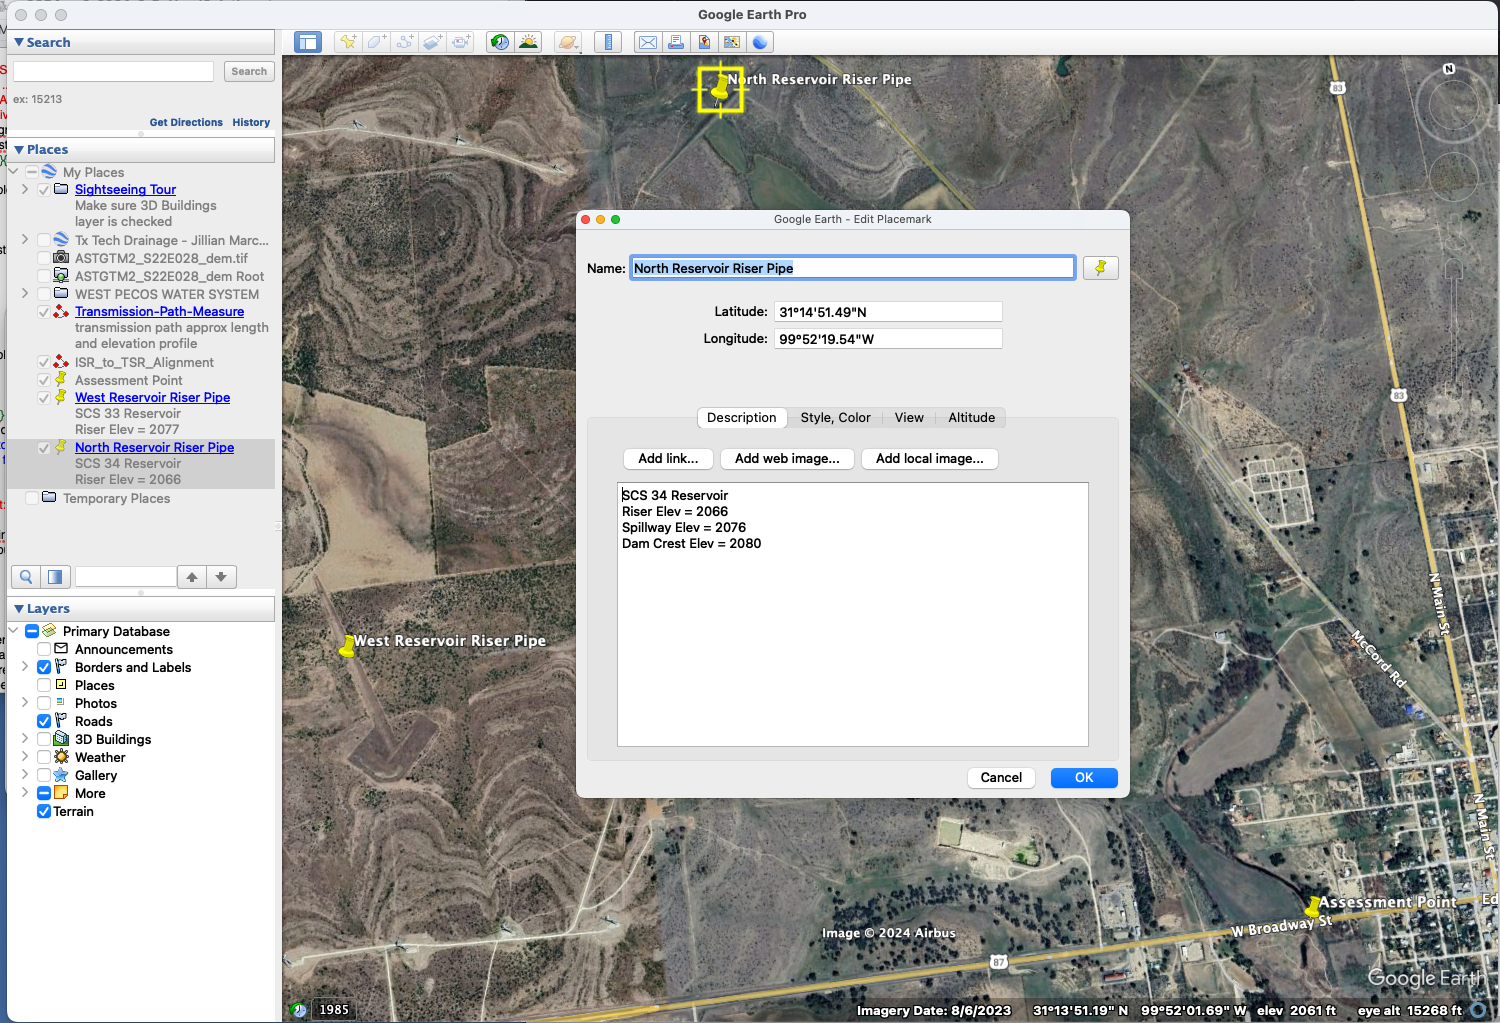
\includegraphics[width=3in]{NorthReservoir.png} 
   \caption{North Reservoir riser pipe location, elevations from USGS 7.5 minute basemap, verfied on Google Earth as "close enough"}
   \label{fig:NorthBasin}
\end{figure}

Then a coordinate transformation as shown in Figure \ref{fig:NorthCoordinates}

\begin{figure}[h!] %  figure placement: here, top, bottom, or page
   \centering
   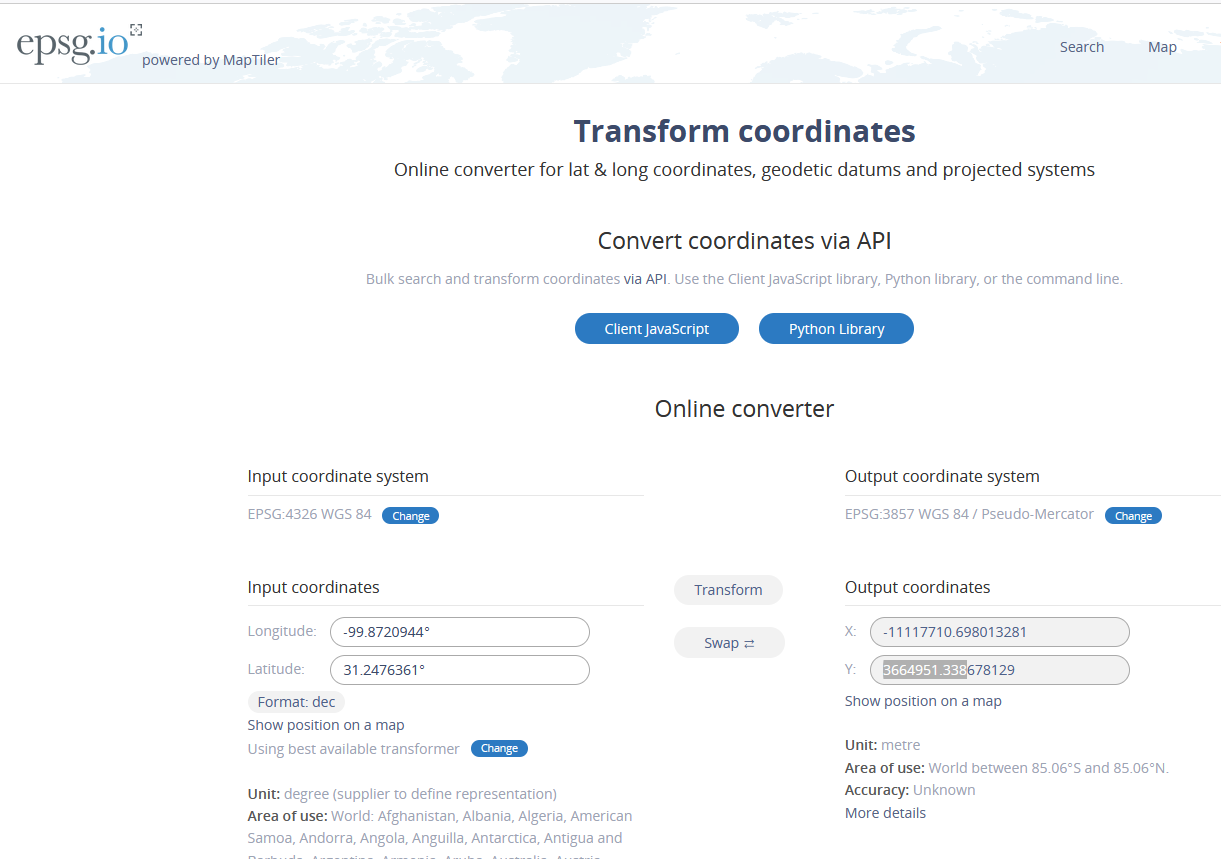
\includegraphics[width=3in]{NorthCoordinates.png} 
   \caption{North Reservoir DMS to UTM conversion}
   \label{fig:NorthCoordinates}
\end{figure}

\clearpage
%%%%%%%%%%%%%%%%%%%%%%%%%%%%%%%%%%%%%%%%%%%%%%%%%%%%%%%%%%%%%%%

Table \ref{tab:SummaryLocations} summarizes the information so far.

% Requires the booktabs if the memoir class is not being used
\begin{table}[htbp]
   \centering
   \caption{Location Summary}
   \begin{tabular}{p{1.5in}p{1.5in}p{1.5in}p{1in}} % Column formatting, @{} suppresses leading/trailing space
Location & Latitude (Northing Meters) & Longitude (Easting Meters) & Elevation (feet) \\
\hline
\hline
Assessment Point& 3660868.901 & -11115601.188 & 2024 \\
~ & ~ & ~ & ~ \\
West Riser Pipe & 3662531.509 & -11119641.472 & 2077 \\
~ & ~ & ~ & ~ \\
North Riser Pipe & 3664951.338 & -11117710.698 & 2066  \\
\hline
\end{tabular}
\label{tab:SummaryLocations}
\end{table}

\clearpage
%%%%%%%%%%%%%%%%%%%%%%%%%%%%%%%%%%%%%%%%%%%%%%%%%%%%%%%%%


\item Determine the channel lengths from the watershed boundary to the SCS impoundments outlets.  

\textbf{By Hand Approach}

Figure \ref{fig:ES2-WatershedArea-3} is a scanned image of the watershed with two possible main channel paths identified.  The longer path would be selected in most instances.  For later work in the project we will need lengths of intermediate channel parts to build the hydrologic model.

\begin{figure}[h!] %  figure placement: here, top, bottom, or page
   \centering
   \includegraphics[width=6in]{Scan2.png} 
   \caption{Study Area -- with grid overlay, outlet (Blue Dot), and subcatchments identified.  Various flow paths are indicted in transparent blue.  1,693 Squares counted to estimate watershed area.  Two long channel paths identified.  Main channel is the longer path (assuming flow passes through the dam).}
   \label{fig:ES2-WatershedArea-3}
\end{figure}

\clearpage
%%%%%%%%%%%%%%%%%%%%%%%%%%%%%%%%%%%%%%%%%%%%%%%%%%%%%%%%%

\item Determine the channel lengths from the SCS impoundment outlets to the junction where the two separate streams combine into the single stream (Hardin Branch).

\textbf{By Hand Approach}
Figure \ref{fig:ES2-WatershedArea-3} is a scanned image of the watershed with two possible main channel paths identified.  Measure the portion from the riser(s) to the junction, and report the result(s).  In this case the distance from the West riser pipe to the junction is about 19 cells, each cell has a diagonal of about 0.14 miles, so the distance is roughly 2.66 miles along the creek path.

For the North riser, the distance to the junction is about 9 cells, each cell has a diagonal of about 0.14 miles, so the distance is roughly 1.26 miles along the creek path.

\clearpage
%%%%%%%%%%%%%%%%%%%%%%%%%%%%%%%%%%%%%%%%%%%%%%%%%%%%%%%%%

\item Determine the channel length from the junction to the Bridge/culvert on US 87.

\textbf{By Hand Approach}
Figure \ref{fig:ES2-WatershedArea-3} is a scanned image of the watershed with two possible main channel paths identified.  Measure the portion from the junction to the outlet, and report the result.  In this case about 18 cells from junction to outlet, each cell has a diagonal of about 0.14 miles, so the distance is roughly 2.52 miles along the creek path.

\clearpage
%%%%%%%%%%%%%%%%%%%%%%%%%%%%%%%%%%%%%%%%%%%%%%%%%%%%%%%%%

\item Determine elevation profiles along the two longest paths.

\textbf{By Hand Approach}


\end{enumerate}

\end{document}  